\documentclass{beamer}

\usepackage[T1]{fontenc}
\usepackage[english]{babel}
\usepackage[utf8]{inputenc}
\usepackage{newunicodechar}
% !TEX spellcheck = en_US

\usetheme[progressbar=frametitle]{metropolis}
\usepackage{appendixnumberbeamer}
\usepackage[percent]{overpic}
\usepackage{multicol}
\usepackage{subfigure}
\usepackage{graphicx}

\title{
	Two-step multi-spectral registration via key-point detector and gradient similarity. \\
	\vspace{1em}
	Application to agronomic scenes for proxy-sensing.
}
\date{\today}
\author{Vayssade Jehan-Antoine}
\institute{\url{jehan-antoine.vayssade@inra.fr}}

\definecolor{OliveGreen}{HTML}{556B2F}

\begin{document}

	\maketitle
	
		\begin{frame}{Material}
			\begin{figure}
				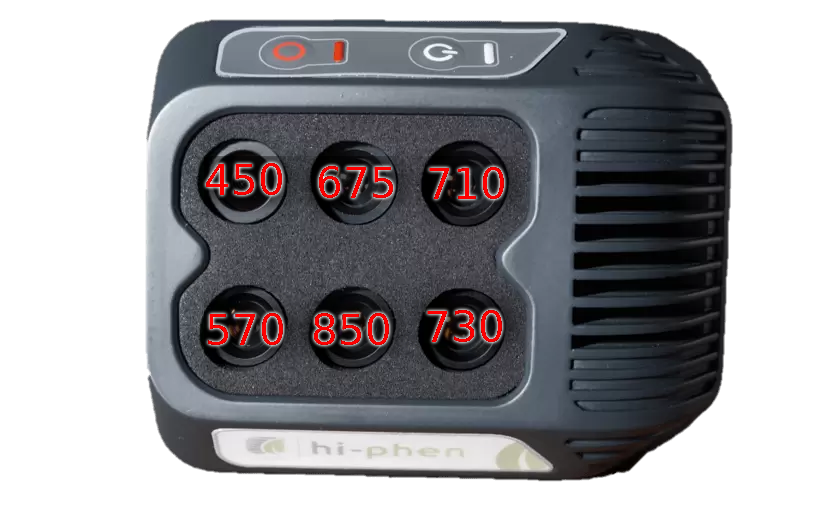
\includegraphics[width=0.4\linewidth]{../figures/airphen-detail4.png}
				\caption{AIRPHEN camera}
			\end{figure}
			\begin{itemize}
				\item interferential filter centered at 450/570/675/710/730/850 nm
				\item focal lens is 8 mm for all wavelength
				\item raw resolution $1280 \times 960$ px with 12 bit of precision.
				\item internal GPS antenna (3D position)
			\end{itemize}
		\end{frame}
	
		\begin{frame}{Data}
			Two dataset was taken, one for calibration, one for evaluation.
			\begin{figure}
				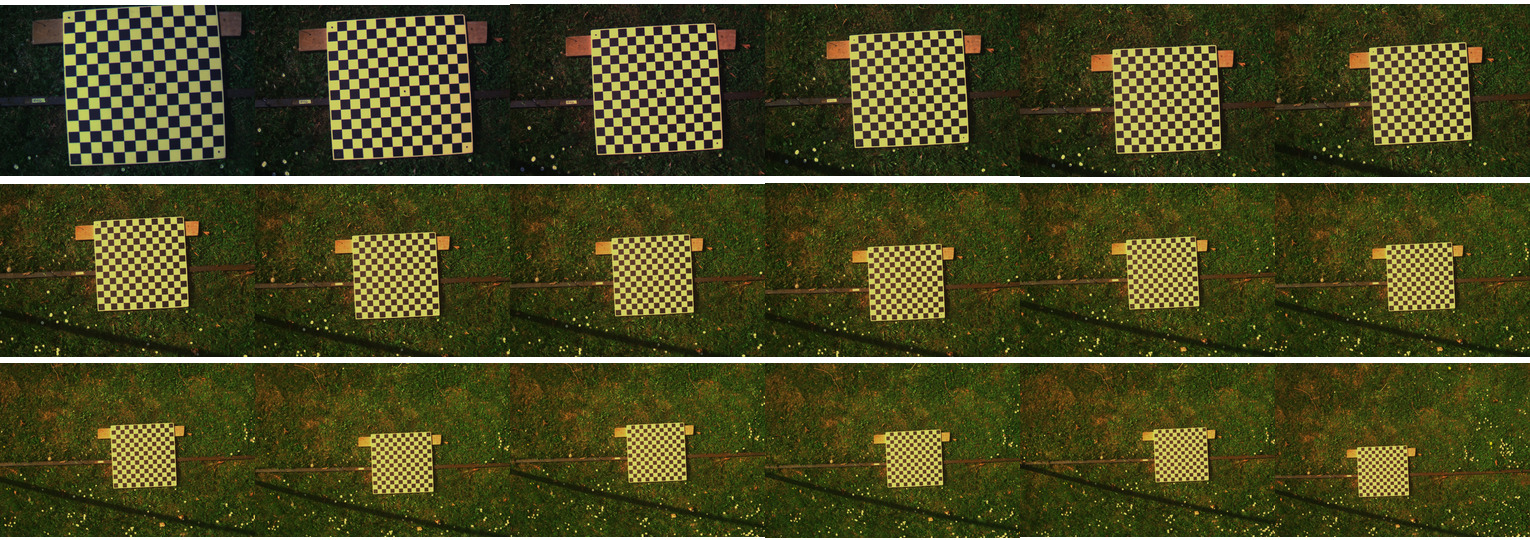
\includegraphics[width=\linewidth]{../figures/calibration-height.jpg}
				\caption{false color reconstruction of each acquisiton height (18) for calibration dataset, from 1.2 to 5 meter.}
			\end{figure}
		\end{frame}
	
	\section{Affine correction}
	
		\begin{frame}{Affine Calibration, translation part}
			\begin{figure}
				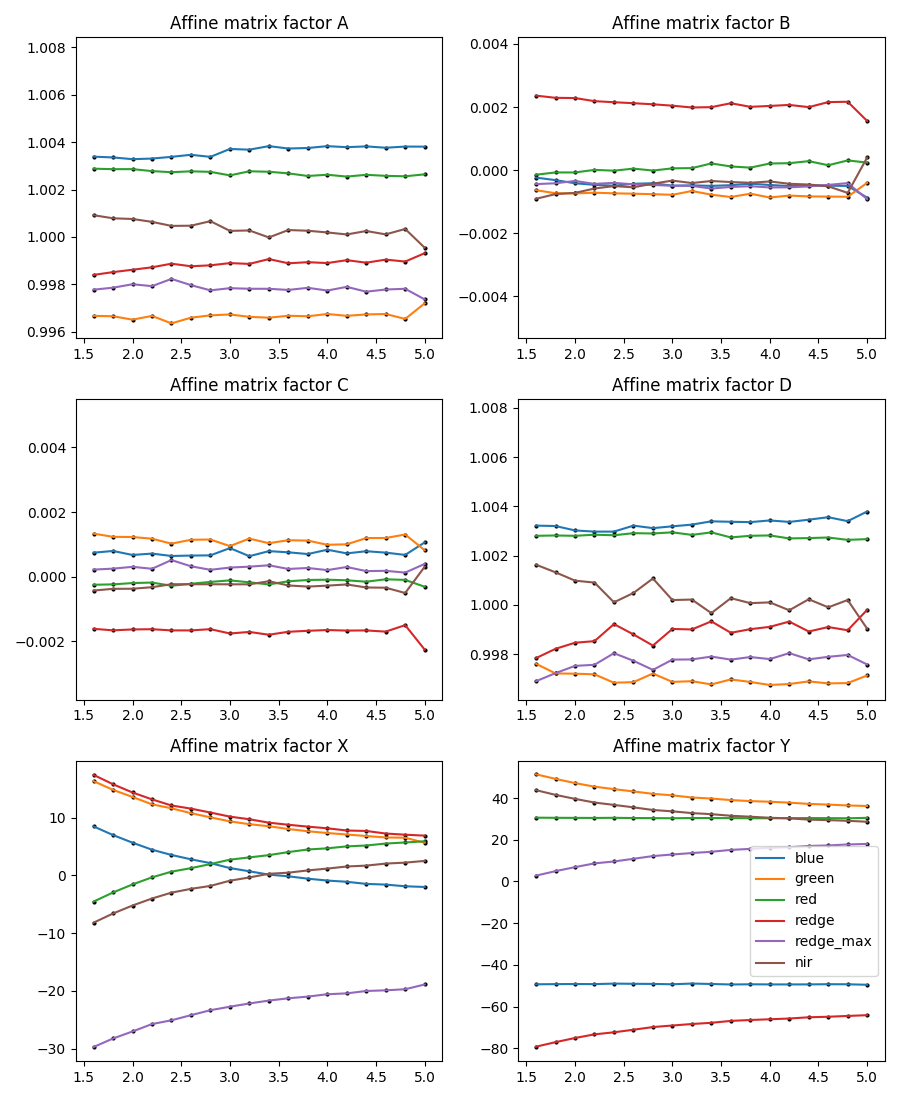
\includegraphics[width=0.7\linewidth]{../figures/affine-translation-height.png}
				\caption{Translation factor from detected chessboard to ``virtual'' center chessboard at each acquisition height, xmax=30, ymax=77}
			\end{figure}
		\end{frame}

		\begin{frame}{Affine Calibration, rotation\&scale part}
			\begin{figure}
				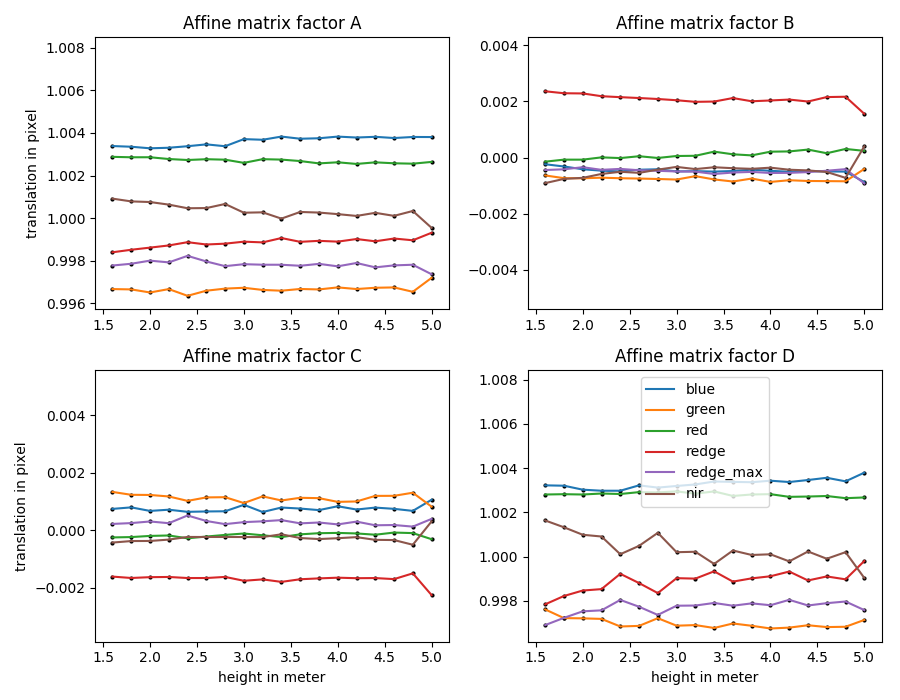
\includegraphics[width=0.7\linewidth]{../figures/affine-rotation-height.png}
				\caption{Rotation and scale factor from detected chessboard to ``virtual'' center chessboard at each acquisition height (precision depend on height but we can notice that these factor are likely invariant)}
			\end{figure}
		\end{frame}
	
		\begin{frame}{Affine Correction}
			From that calibration a new affine matrix are build:
			
			\begin{itemize}
				\item For $X,Y$ factors an equation are fit \footnote{Levenberg-Marquardt with linear least squares regression} and the height from the GPS are used to get the nearest correction
				\begin{itemize}
					\item $t = \alpha h^3 + \beta h^2 + \theta h + \gamma$
				\end{itemize}
				\item For $A,B,C,D$ the values at the most accurate height are used
			\end{itemize}
		
			Each spectral band is warped using the corresponding affine transformation.
			And a crop are applied.
		\end{frame}
	
	\section{Perspective correction (refinement)}
		\begin{frame}{Gradient transform for keypoint detection}
			To optimize the search of specific keypoint such as gradient break,
			each spectral band are transformed :
			\begin{itemize}
				\item normalizing using Gaussian blur $I/(G+1)*255$ 
				\item gradient is computed with the sum of absolute Sharr filter
				\item normalization using CLAHE to locally improve their intensity
			\end{itemize}
		\end{frame}
	
		\begin{frame}{Keypoint detector (9)}
			\begin{itemize}
				\item (ORB) Oriented FAST and Rotated BRIEF
				\item (AKAZE) Fast explicit diffusion for accelerated features in nonlinear scale spaces
				\item (KAZE) A novel multi-scale 2D feature detection and description algorithm in nonlinear scale spaces
				\item (BRISK) Binary robust invariant scalable key-points
				\item (AGAST) Adaptive and generic corner detection based on the accelerated segment test
				\item (MSER) maximally stable extremal regions
				\item (SURF) Speed-Up Robust Features
				\item (FAST) FAST Algorithm for Corner Detection
				\item (GFTT) Good Features To Track
			\end{itemize}
		\end{frame}
	
		\begin{frame}{Perspective correction via Keypoint}
			\begin{figure}
				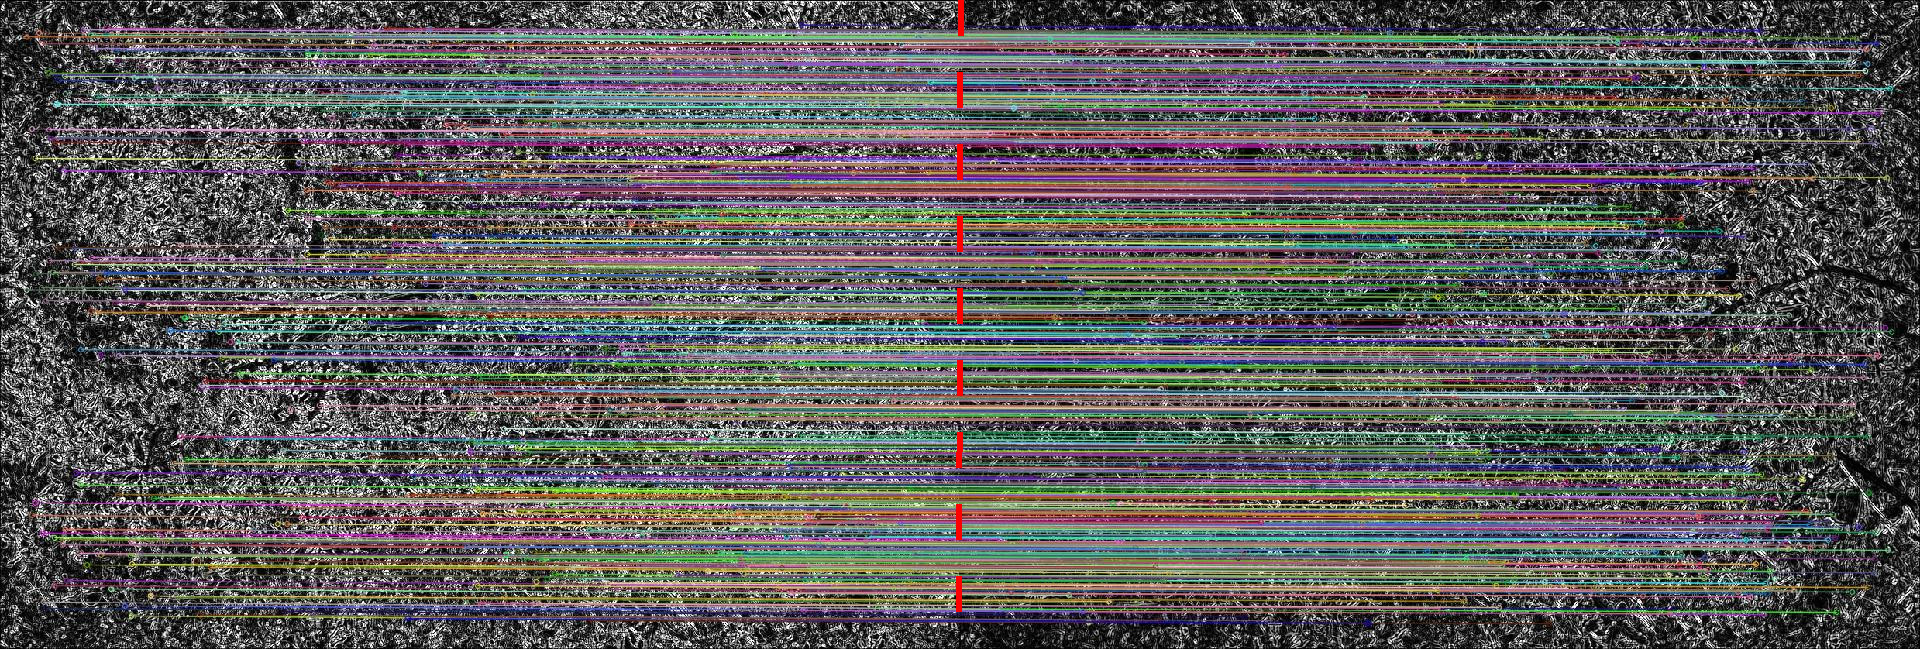
\includegraphics[width=\linewidth]{../figures/prespective-feature-matching}
				\caption{Bruteforce keypoint matching in normalized gradient and filtering (570nm left \& 850nm right)}
			\end{figure}
		\end{frame}
	
		\begin{frame}{Results}
			\begin{figure}
				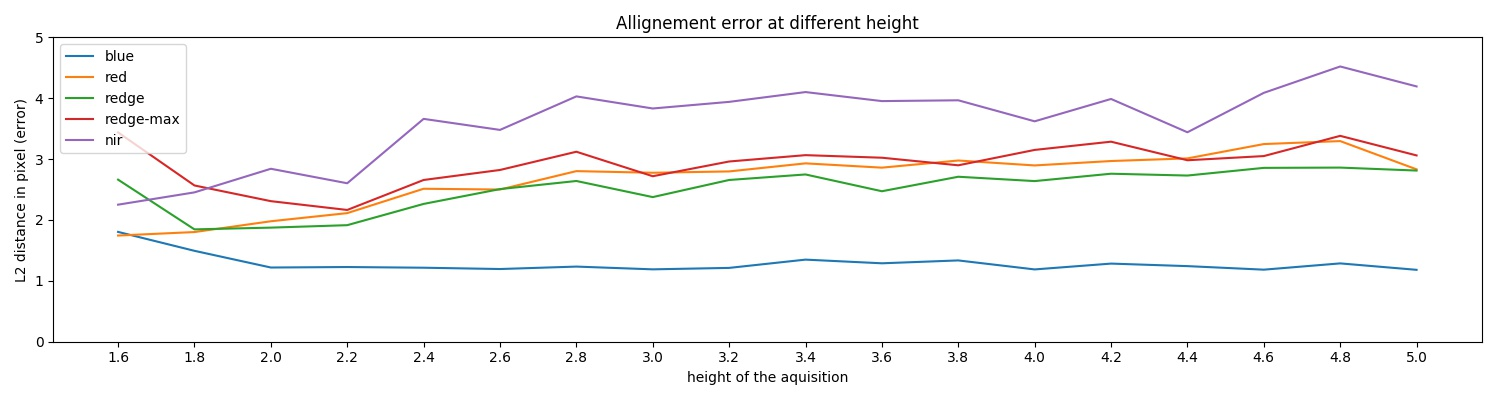
\includegraphics[width=0.8\linewidth]{../figures/affine-allignement-rmse.jpg} \\
				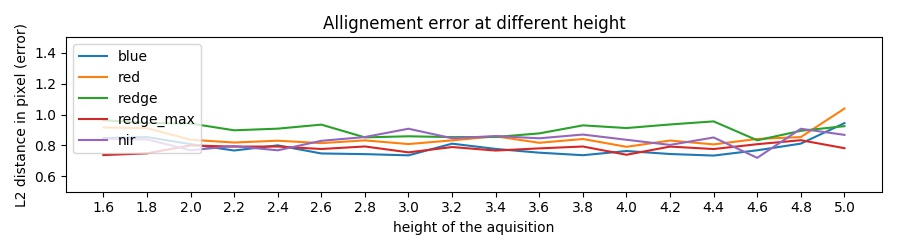
\includegraphics[width=0.8\linewidth]{../figures/prespective-allignement-rmse.jpg}
				\caption{Performance evaluation with 570nm as reference}
			\end{figure}
		\end{frame}
			
\end{document}